\documentclass[a4paper,10pt]{article}
\usepackage[ngerman]{babel}
\usepackage[utf8]{inputenc}
\usepackage[a4paper,vmargin={20mm,20mm},hmargin={20mm,10mm}]{geometry}
\usepackage[T1]{fontenc}

\usepackage{tocloft, multicol} 
\usepackage{amsmath, amsfonts, amssymb} 
\usepackage{booktabs} 
\usepackage{bm}  
\usepackage{caption}
\usepackage{subcaption}
\usepackage{enumitem}
\usepackage{graphicx} 
\usepackage{listings}
\usepackage{mathtools}
\usepackage[dvipsnames]{xcolor}
\usepackage{wrapfig,lipsum,threeparttable}
\usepackage{footmisc, fixfoot}



\DeclareFixedFootnote{\fnrefa}{ P. T. Boggs and J. E. Rogers, “Orthogonal Distance Regression,” in “Statistical analysis of measurement error models and applications: proceedings of the AMS-IMS-SIAM joint summer research conference held June 10-16, 1989,” Contemporary Mathematics, vol. 112, pg. 186, 1990. }
\DeclareFixedFootnote{\fnrefb}{ Dr. J.Wagner - Physikalisches Anfängerpraktikum - V. 1.1 Stand 1/2018, Versuch 221}


\lstset{literate=%
    {Ö}{{\"O}}1
    {Ä}{{\"A}}1
    {Ü}{{\"U}}1
    {ß}{{\ss}}1
    {ü}{{\"u}}1
    {ä}{{\"a}}1
    {ö}{{\"o}}1
    {~}{{\textasciitilde}}1
}
\lstset{%
backgroundcolor=\color{gray!32},
basicstyle=\ttfamily\footnotesize,
numbers=left,numberstyle=\scriptsize,
frame=single,
breaklines=true,
}

\usepackage[wby]{callouts}
\title{WS19/20, PAP2.1, Versuch 221:\\ Adiabatenkoeffizient}
\date{Versuchsdurchführung: \\29. Oktober, 2019}
\author{Praktikanten:\\Gerasimov, V. \& Reiter, L.\\\\Betreuer:\\ Neitzel, C.}


\begin{document}

\maketitle

\newpage

\tableofcontents

\addtocontents{toc}{~\hfill\textbf{Seite}\par}

\section{Einführung}\boldmath
Der Adiabatenexponent ist das Verhältnis der spezifischen Wärmekapazität bei konstantem Druck zu der spezifischen Wärmekapazität bei konstantem Volumen:
\begin{equation}
\kappa=c_p / c_V
\end{equation}
\(\kappa\) ist der Exponentialkoeffizient im Poisson'schen Gesetz \eqref{eq:poisson}. Ist \(f\) die Zahl der Freiheitsgrade des Moleküls, so liefert die kinetische Gastheorie die Beziehung \eqref{eq:dof}.
\begin{equation}\label{eq:poisson}
\boxed{p V^{\kappa} = konst.}
\end{equation}
\begin{equation}\label{eq:dof}
\kappa= 1 + \frac{2}{f}
\end{equation}
Bei genügend niedrigen Temperaturen kommt es zum Einfrieren von Freiheitsgraden und diese  eingefrorene Freiheitsgrade Tragen dann nicht zum Adiabatenexponenten bei. Daraus folgen als Näherungswerte, die in Wirklichkeit temperaturabhängig sind, die Zahlenwerte
\[\kappa = 5/3 \approx 1.67\]
für einatomige Gase,
\[\kappa = 7/5 = 1.4\]
für zweiatomige Gase und
\[\kappa = 4/3 \approx 1.33\]
für drei- und mehratomige Gase.\\
In diesem Versuch wollen wir zusteuert \(\kappa_{Luft}\) bestimmen mit Hilfe der Messung des Adiabatenkoeffizienten nach Clément \& Desormes.
Danach bestimmen wir \(\kappa_{Luft}\) ein zweites Mal Hilfe einer Messung nach Rüchhardt. Diese Messmethode wiederholen wir für Argon. Somit habe wir 2 Messmethoden für den Adiabatenexponenten der Luft, die wir miteinander und Literaturwerten vergleichen können. Für Argon werden wir also nur 1 Messergebiss haben, dass wir aber auch mit Literaturwerten vergleichen können.

\section{Versuchsaufbau, Literaturwerte \& Vorbereitung}
Literaturwerte\footnote{ Engineering ToolBox, (2004). Air - Specific Heat at Constant Pressure and Varying Temperature. [online] Available at: https://www.engineeringtoolbox.com/air-specific-heat-capacity-d\_705.html [Accessed 10/12/2019]}'\footnote{ Engineering ToolBox, (2003). Specific Heat and Individual Gas Constant of Gases. [online] Available at: https://www.engineeringtoolbox.com/specific-heat-capacity-gases-d\_159.html [Accessed 10/12/2019]} zum späteren Vergleich:
\begin{align*}
\kappa_{Luft,Literatur}&=1.402(1)\\
\kappa_{Argon,Literatur}&=1.648(1)
\end{align*}
Skizzen zu beiden Versuchsbauten sind in Abb.\ref{fig:aufbau1} und Abb.\ref{fig:aufbau2} dargestellt.\\
Die Werte für \(V\), \(m\) und \(d=2r\) und ihre angegebenen Messunsicherheiten an den Versuchsaufbauten nach Rüchhardt wurden in Tabelle \ref{tab:Tab2} übertragen. Außerdem benötigen wir ein Manometer um den Luftdruck\(p\)  im Raum während der Versuchsdurchführung zu messen.

\section[Herleitungen der verwendeten Formeln]{Herleitungen der verwendeten Formeln\fnrefb}
\begin{wrapfigure}{l}{0.38\textwidth}
  \centering
  \caption{pV-Diagramm zu Messung nach Rüchhardts}
  \begin{annotate}{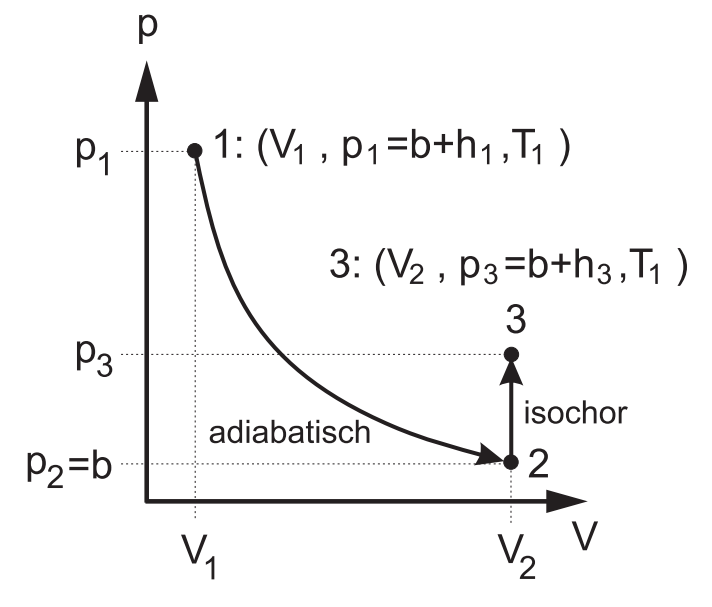
\includegraphics[width=0.38\textwidth]{pv.png}}{1}
  \end{annotate}

\label{fig:pv}
\end{wrapfigure} 
\subsection{Messung des Adiabatenkoeffizienten nach Rüchhardt}
Der Messaufbau ist in Abbildung \ref{fig:aufbau1} dargestellt.\\\\
Der Druck im luftgefüllten Gasbehälter lässt sich mit Hilfe des Luftbalgs vergrößern und kann am Manometer abgelesen werden. Zuerst wird ein Überdruck im Gasbehälter erzeugt, durch Pumpen mit dem Luftbalg. Die Luft dabei erwärmt dabei. Wartet man nun so lange ab, bis sich das Gas wieder auf Zimmertemperatur abgekühlt hat, so ist der Zustand 1 im pV-Diagramm in Abbildung \ref{fig:pv} erreicht:
\begin{equation}
  \text{Zustand 1:}\quad V_1,\quad p_1=b+h_1, \quad T_1
\end{equation}
wobei \(V_1\) das Volumen im Zustand 1, \(b\) der äußere Luftdruck, \(h_1\) die Höhendifferenz des Manometers und \(T_1\) die Temperatur des Gases im Zustand 1 (Zimmertemperatur) bezeichnen. \\ Im nächsten Schritt wird der Gasauslassstopfen am Gasbehälter für eine relativ kurze Zeit geöffnet, sodass sich der Druck \(p\) im Behälter dem äußeren Luftdruck \(b\) angleicht. Dabei entweichen Moleküle aus der Flasche, d.h. die Gasmenge ändert sich. Dies ist gleichbedeutend mit der Annahme, dass man durch eine Volumenvergrößerung um \(\Delta V\) zu dem Druck \(b\) kommt. Da der Druckausgleich sehr schnell erfolgt, findet kein Wärmeaustausch mit der Umgebung statt. Es handelt sich daher um einen adiabatischen Prozess, bei dem sich die Temperatur des Gases um \(\Delta T\) abkühlt. Für den Zustand 2 des Gases gilt dann:
\begin{equation}
  \text{Zustand 2:}\quad V_2= V_1+ \Delta V,\quad p_2=b, \quad T_2=T_1 - \Delta T
\end{equation}
\begin{figure}[htb]
  \centering
  \begin{subfigure}{0.48\textwidth}
  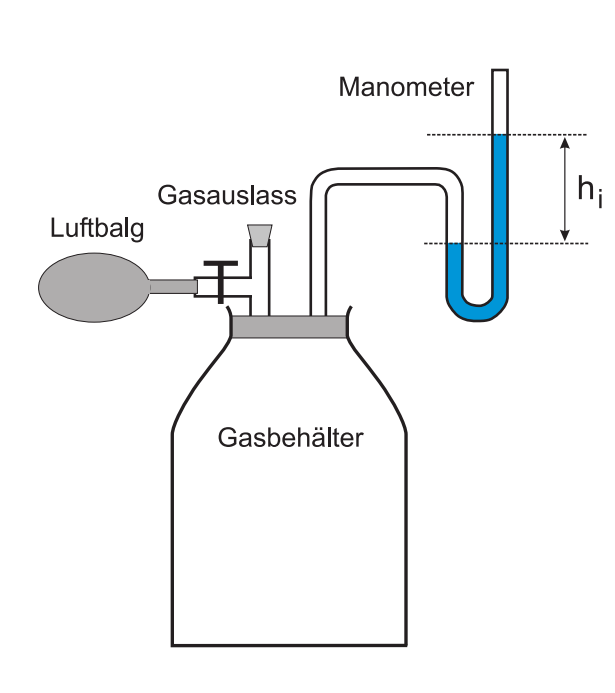
\includegraphics[width=1\linewidth]{pic1.png}
  \caption{Skizze des Aufbaus nach Clément und Desormes.}
\label{fig:aufbau1}
  \end{subfigure}
    \begin{subfigure}{0.48\textwidth}
 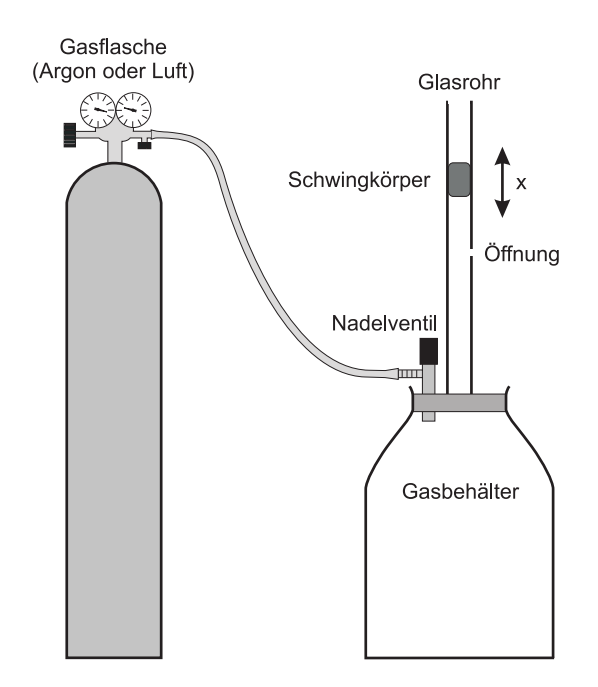
\includegraphics[width=1\linewidth]{pic2.png}
 \caption{Skizze des Aufbaus nach Rüchhardt. Bei uns in zweifacher Ausführung: ein Mal mit Luft und ein Mal mit Argon.}
\label{fig:aufbau2}
  \end{subfigure}
 \caption[Versuchsaufbau]{Versuchsaufbau\footnotemark}
\end{figure}\footnotetext{ Dr. J.Wagner - Physikalisches Anfängerpraktikum - V. 1.1 Stand 1/2018, Versuch 221}

Danach warten wir  solange ab, bis die Temperatur des Gases wieder auf Zimmertemperatur angestiegen ist. Da sich dabei \(V\) ändert, handelt es sich um eine isochore Zustandsänderung bei der der Druck im Gasbehälter ansteigt. Wenn die Temperatur des Gases schließlich Zimmertemperatur erreicht hat, befindet sich die Luft im Zustand 3:
\begin{equation}
  \text{Zustand 3:}\quad V_3=V_2= V_1+ \Delta V,\quad p_3=b+h_3, \quad T_3=T_1
\end{equation}
Die Zustände 1 und 2 sind durch die Poisson'sche Gleichung \eqref{eq:poisson} miteinander verknüpft:
\begin{equation}
  p_1{V_1}^{\kappa}=p_2{V_2}^{\kappa}
\end{equation}
woraus folgt, dass
\begin{equation} \label{eq:gl5}
  \left(b+h_1\right){V_1}^{\kappa}=p_2{\left(V_1+\Delta V\right)}^{\kappa}
\end{equation}
Da \(\Delta V \ll V_1\) ist können wir \(\left(V_1 + \Delta V \right)^{\kappa}\) nähern durch
\begin{equation*}
  \left(V_1 + \Delta V \right)^{\kappa} = {V_1}^{\kappa} \left(1+ \frac{\Delta V}{V_1}\right)^{\kappa} 
\end{equation*}
\begin{equation} 
  \approx  {V_1}^{\kappa} \left(1+{\kappa} \frac{\Delta V}{V_1}\right)
\end{equation}
Setzen wir diesen Ausdruck in Gleichung \eqref{eq:gl5} ein, so erhalten wir
\begin{equation} \label{eq:gl7}
  \frac{h_1}{b} = \kappa \frac{\Delta V}{V_1}
\end{equation}

In den Zuständen 1 und 3 ist die Temperatur \(T_1=T_3\) der Luft im Gasbehälter gleich, d.h. es gilt das Boyle-Mariotte'sche Gesetzt:
\begin{equation} 
  \text{Wenn}\quad n= konst.\quad \text{und} \quad T=konst.  \quad \text{, dann}\quad  pV=konst.
\end{equation}
\begin{equation} 
  \implies p_1 V_1 = p_3 V_3
\end{equation}
\begin{equation} 
  \implies \left(b+h_1\right) V_1 = \left(b+h_3\right) \left(V_1 + \Delta V\right)
\end{equation}
Da \(h_3 \ll b\) und \(\Delta V \ll V_1\), kann der Term \(h_3 \left(\Delta V\right)\) vernachlässigt werden. Somit
ergibt sich:
\begin{equation}
  \frac{\Delta V}{V_1}= \frac{h_1 - h_3}{b}
\end{equation}
Wir setzen diesen Ausdruck in Gleichung \eqref{eq:gl7} ein, und erhalten schließlich:
\begin{equation} \label{eq:kappa_1}
  \boxed{\kappa = \frac{h_1}{h_1-h_3} }
\end{equation}
\subsection{ Messung des Adiabatenkoeffizienten nach Clément \& Desormes}
Eine weitere Bestimmung des Adiabatenkoeffizienten eines Gases, ist mit der Methode nach Rüchardt möglich (Abbildung \ref{fig:aufbau2}). Auf einem Gasbehälter ist eine Glasröhre montiert. Bringt man in das Glasrohr einen Schwingkörper, der nahezu den gleichen Durchmesser \(d =2r\) wie das Glasrohr besitzt, so schwingt
dieser in der Röhre auf und ab. Dabei wird das Gas periodisch adiabatisch komprimiert und expandiert. Allerdings ist die Schwingung stark gedämpft, sodass nur wenige Perioden beobachtbar sind. Um dem entgegenzuwirken befindet sich in der Mitte das Glasrohrs eine kleine Öffnung von ungefähr 1 mm Durchmesser. Lässt man einen gleichmäßigen Gasstrom in die Flasche, dann wirkt, sofern sich der Schwingkörper unterhalb der Öffnung befindet, ein zusätzlicher Druck auf den Schwingkörper. Befindet sich der Schwingkörper über der Öffnung, so entweicht der Gasstrom durch die Öffnung und der Druck sinkt. Wir beachten, dass durch diese Maßnahme nur die Reibungsverluste ausgeglichen werden. Die eigentliche Bewegung des Schwingkörpers beruht auch weiterhin auf die adiabatische Kompression und
Expansion des Gases.\\\\
Der Schwingkörper befindet sich im Gleichgewicht wenn der Druck \(p\) in der
Flasche gleich der Summe aus dem Luftdruck\(p_0\) und dem \glqq Schweredruck\grqq~des
Schwingkörpers ist:
\begin{equation}
  p=p_0 \frac{mg}{A}
\end{equation}
wobei \(m\) die Masse und \(A\) die Querschnittsfläche des Schwingkörpers beschreiben. Schwingt der Körper um eine kleine Strecke \(x\) über die Gleichgewichtslage hinaus, wobei sich der Druck \(p\) um \(dp\) ändert, so gilt nach dem Newton'schen Gesetz:
\begin{equation} \label{eq:gl14}
 m \frac{{d^2}x}{{dt}^2}=A\:{dp}
\end{equation}
Da der Vorgang adiabatisch erfolgt, gilt die Poisson'sche Gleichung \eqref{eq:poisson}
\begin{equation}\tag{\ref{eq:poisson}}
p V^{\kappa} = konst.
\end{equation}
Differentiaton dieses Ausdrucks nach \(V\)  liefert:
\begin{equation}
p V^{\kappa} = V^{- \kappa} \times konst.
\end{equation}
\begin{equation}
\frac{dp}{dV} = - \kappa V^{-\kappa -1 } \times konst.
\end{equation}
\begin{equation}
\frac{dp}{dV} = - \kappa \frac{p}{V}
\end{equation}
\begin{equation}
\frac{dp}{dV} = - \kappa \frac{p}{V}\: dV
\end{equation}
Setzen wir diesen Ausdruck in Gleichung \eqref{eq:gl14} ein, so erhalten wir:
\begin{equation}
 m \frac{{d^2}x}{{dt}^2}= - A \kappa \frac{p}{V}\:{dV}
\end{equation}
Mit \(dV = Ax = \pi r^2 x\), wobei \(r=d/2\) den Radius des Glasrohrs darstellt, ergibt sich:
\begin{equation}
 m \frac{{d^2}x}{{dt}^2}= - \pi^2 r^4\kappa \frac{p}{V} x
\end{equation}
bzw.
\begin{equation} \label{eq:gl22}
 \ddot{x} + \frac{\pi^2 r^4 \kappa p}{mV} x = 0
\end{equation}
Gleichung \eqref{eq:gl22} ist die Bewegungsgleichung eines harmonischen Oszillators. Die
allgemeine Form lautet
\begin{equation} 
 \ddot{x} + \omega^2 x = 0
\end{equation}
Vergleichen wir dies mit Gleichung \eqref{eq:gl22}, so ergibt sich für die Kreisfrequenz \(\omega\) des Schwingkörpers:
\begin{equation} 
 \omega = \sqrt{\frac{\pi^2 r^4 \kappa p}{mV}}
\end{equation}
bzw. fur die Periodendauer \(T\)
\begin{equation} 
 T = \sqrt{\frac{4mV}{ r^4 \kappa p}}
\end{equation}
Für den Adiabatenkoeffizienten \(\kappa \) folgt dann:
\begin{equation} \label{eq:kappa_2}
\boxed{\kappa = \frac{4 m V}{r^4 T^2 p}}
\end{equation}

\section{ Versuch nach Clément \& Desormes}
\subsection[Durchführung]{Durchführung\fnrefb}
Durch mehrmaliges Pumpen mit dem Luftbalg erzeugen wir einen Überdruck im Gasbehälter. Während diesem Vorgang erwärmt sich drinnen die Luft. Wir warten daher nach der Druckerhöhung 3-5 Minuten ab, bis die Temperatur des Gases wieder auf Zimmertemperatur abgesunken ist. Das Erreichen der Zimmertemperatur lässt am asymptotischen Absinken des Druckes am
Manometer auf den Endwert \(h_1\) überprüfen. Dies entspricht, wie im Kapitel \glqq Herleitung\grqq~erläutert, dem Zustand 1 im pV-Diagramm (Abb.\ref{fig:pv}. Bei jedem Messdurchgang notieren wir den Wert für \(h_1\).\\\\
Danach öffnen wir für etwa 2 Sekunden den Stopfen der Gasauslassöffnung. Dadurch wird ein adiabatischer Druckausgleich erzielt (Zustand 2 im pV-Diagramm) und warten anschließend wieder den Temperaturausgleich ab, bis sich ein konstanter Überdruck \(h_3\) eingestellt hat (Zustand 3). Bei jedem Messdurchgang notieren wir diesen Wert für \(h_3\) auch.\\\\
Der Versuch wird 5 Mal wiederholt. Falls der Enddruck \(h_3\) 
noch groß genug ist, kann man diesen Zustand als Anfangszustand für
die folgende Messung benutzen. Das war aber bei uns nie der Fall, und wir mussten jedes Mal den Druck durch Pumpen mit dem Luftbalg erneut erhöhen.

\subsection{Messergebnisse}
Messdaten wurden dem Versuchsprotokoll (29. Oktober, 2019) entnommen und in Tabelle \ref{tab:Tab1} übertragen.
\unboldmath
\begin{table}[htb]
\centering
\caption{Messung der Drucks}\label{tab:Tab1}
\begin{threeparttable}
\begin{tabular}{rr}
\toprule
Startdruck \boldmath\(h_1\)\unboldmath & Enddruck \boldmath\(h_3\)\unboldmath \\
\([mm]\)&\([mm]\)\\
\midrule
\(102\pm2\)&\(25\pm2\)\\
\(90\pm2\)&\(23\pm2\)\\
\(122\pm2\)&\(27\pm2\)\\
\(37\pm2\)&\(9\pm2\)\\
\(69\pm2\)&\(15\pm2\)\\
  \bottomrule
 \end{tabular}
\begin{tablenotes}
\raggedright
\item[1]sowohl \boldmath\(\Delta h_1\) als auch \(\Delta h_3 \) sind abgeschätzt als ganze Skaleneinteilung am Manometer\unboldmath
\end{tablenotes}
\end{threeparttable}\end{table}
\boldmath
\subsection{Kurvenanpassung mit Python}
\subsubsection{Source Code \& Input}
Den Adiabatenkoeffizienten nach Clément \& Desormes können wir direkt aus den Werten \(h_1 \)  und \(h_3 \) mit Hilfe von Gleichung \eqref{eq:kappa_1} berechnen:
\begin{equation}\tag{\ref{eq:kappa_1}}
\kappa = \frac{h_1}{h_1-h_3} 
\end{equation}
\begin{equation*}
\Delta \kappa = \kappa \left(\frac{\Delta \left(\kappa^{-1}\right)}{\kappa^{-1}}\right) = {\kappa^2 }\left( \Delta \left(1-\frac{h_3}{h_1}\right)\right)
\end{equation*}
\begin{equation*}
= \left({\frac{h_1}{h_1-h_3}} \right)^2 \left( \frac{h_3}{h_1} \sqrt{{\left(\frac{\Delta  h_1}{h_1}\right)^2}+{\left(\frac{\Delta  h_3}{h_3}\right)^2}}\right) 
\end{equation*}
\begin{equation} \label{eq:Deltakappa_1}
= {\frac{h_1 h_3}{\left( h_1-h_3 \right)^2}} \sqrt{{\left(\frac{ \Delta  h_1}{h_1}\right)^2}+{\left(\frac{ \Delta h_3}{h_3}\right)^2}}
\end{equation}
Wir gehen davon aus, dass der Adiabatenkoeffizient für ein gegebenes Gas und den von uns betrachteten Temperaturbereich konstant ist.
Daher ist unser funktionales Modell für die Ausgleichungsrechnung wie folgt:
\begin{equation} \label{eq:Fit1}
	\kappa = konst.
\end{equation} 
So sieht unsere Python-Implementierung aus:\\

Header:
\begin{lstlisting}
%matplotlib inline
import matplotlib.pyplot as plt
import numpy as np
from scipy.stats import chi2
from decimal import Decimal

def format_e(n):
    a = '%e' % Decimal(n)
    return a.split('e')[0].rstrip('0').rstrip('.')+'e'+a.split('e')[1]

\end{lstlisting}

Messwerte aus Tabelle \ref{tab:Tab1} in mm:\begin{lstlisting}
h_1 = np.array([102,90,122,37,69])
Fehler_h_1 = np.array([2,2,2,2,2])

h_3 = np.array([25,23,27,9,15])
Fehler_h_3 = np.array([2,2,2,2,2])

\end{lstlisting}

Berechnung des Adiabatenkoeffizienten  \(\kappa_{Luft,1}\) und \(\Delta \kappa_{Luft,1}\) nach \eqref{eq:kappa_1} bzw. \eqref{eq:Deltakappa_1}:\begin{lstlisting}
kappa_Luft_1 = h_1/(h_1-h_3)
Fehler_kappa_Luft_1 = (h_1*h_3/((h_1-h_3)**2))*np.sqrt((Fehler_h_1/h_1)**2+2*(Fehler_h_3/h_3)**2)

\end{lstlisting} 

Nummerierung (um es später darstellen zu können): \begin{lstlisting}
n = np.linspace(1,kappa_Luft_1.size,kappa_Luft_1.size)
Fehler_n = 1

\end{lstlisting}

Fitfunktion \eqref{eq:Fit1} wird deklariert:\begin{lstlisting}
from scipy import odr

def fit_func(p, x):
    (c) = p
    return x*0+c

model = odr.Model(fit_func)

\end{lstlisting}

darzustellende Daten werden übergeben:\begin{lstlisting}
x = n
y = kappa_Luft_1
delta_x = Fehler_n
delta_y = Fehler_kappa_Luft_1

\end{lstlisting}

Startparameter für Ausgleichungsrechnung werden gesetzt, sodass Lösung konvergiert:\begin{lstlisting}
para0 = [0]

data = odr.RealData(x, y, sx=delta_x, sy=delta_y)
odr = odr.ODR(data, model, beta0=para0 )
out = odr.run()

\end{lstlisting}

Endgültige Ausgleichungsparameter und ihre Kovarianzmatrix werden ausgelesen:\begin{lstlisting}
popt = out.beta
perr = out.sd_beta

\end{lstlisting}

Der Chi-Quadrat-Test wird durchgeführt unter Berücksichtigung von \( \Delta h_1\) und \(\Delta h_3\). D.h.~es wird jeweils der senkrechte/orthogonale Abstand der Messwerte zur Fitfunktion (Abb.\ref{fig:chi}) berechnet und normiert\fnrefa.
 Die Summe der normierten Abstandsquadrate, der \unboldmath\( \chi^{2}\)-Wert, wird  reduziert.\boldmath

\begin{figure}[htb]
  \centering
  \begin{annotate}{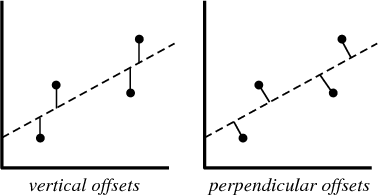
\includegraphics[width=0.5\textwidth]{chi.png}}{1}
  \end{annotate}
\caption[Abstände von Messdaten zur Fitfunktion]{Abstände von Messdaten zur Fitfunktion\footnotemark}
\label{fig:chi}
\end{figure}
\footnotetext{http://mathworld.wolfram.com/LeastSquaresFitting.html}

\begin{lstlisting}
dof = x.size-popt.size
chisquare = out.sum_square
chisquare_red = chisquare/dof
prob = round(1-chi2.cdf(chisquare,dof),2)*100

\end{lstlisting}

Auslesen der Messergebnisse:\begin{lstlisting}
kappa_Luft_1_mean = popt[0]
Fehler_kappa_Luft_1_mean = perr[0]

\end{lstlisting}

Ausgabe der Messergebnisse wird erstellt:\begin{lstlisting}
print('1.Messmethode:')
print('kappa_Luft =', format_e(kappa_Luft_1_mean), ' +- ', format_e(Fehler_kappa_Luft_1_mean))
print('Chi-Quadrat =', chisquare)
print('Freiheitsgrade =', dof)
print('Chi-Quadrat reduziert =', chisquare_red)
print('Wahrscheinlichkeit ein größeres oder gleiches Chi-Quadrat zu erhalten =', prob, '%')

\end{lstlisting}

\subsubsection{Output}
\begin{lstlisting}
1.Messmethode:
kappa_Luft = 1.305408e+00  +-  1.269561e-02
Chi-Quadrat = 1.06472768776082
Freiheitsgrade = 4
Chi-Quadrat reduziert = 0.266181921940205
Wahrscheinlichkeit ein größeres oder gleiches Chi-Quadrat zu erhalten = 90.0 %
\end{lstlisting}
Wir erfahren also sofort, dass
\begin{align*}
{\kappa_{Luft,1}}&=1.305(13)
\end{align*}
und als Ergebnis auf unseren Anpassungstest:
\[\chi^{2}_{red}=1.1\]
Die Wahrscheinlichkeit ein größeres oder gleiches Chi-Quadrat zu erhalten ist
 \[P\approx  90.0 \%\]
und später werden alle Messdaten und der Fit in  Abb.\ref{fig:Fig1} dargestellt.
\subsection{Auswertung}
Wie in Abbildung \ref{fig:Fig1} zu sehen ist, liegen manche Messungen zwar in der 1-Sigma Umgebung vom Literaturwert \(\kappa_{Luft,Literatur}=1.402(1)\), jedoch weicht unser Mittelwert stark von ihm ab:
\[\frac{{kappa_{Luft,1}}-{kappa_{Luft,Literatur}}}{\Delta {kappa_{Luft,1}}}=7.5\]
Die Wahrscheinlichkeit ein größeres oder gleiches Chi-Quadrat zu erhalten \(P\approx  90.0 \%\) ist komplett in Ordnung. Also passen unsere statistischen Fehler zum theoretischem Modell \eqref{eq:Fit1} einer Konstanten.
Diese 7-Sigma-Abweichung ist wahrscheinlich ein Resultat von geringen statistischen Fehlern, die alle Beachtet wurden, und einem oder mehren systematischen Fehlern die vergessen oder nicht beachtet worden sind. Zum Beispiel konnte es sein, dass die Zeit beim abwarten des Temperaturausgleichs nicht lang genug war oder beim Ablesen des Manometers wurde nicht korrekt die Perspektive beachtet, weswegen Ablesewerte in verschiedenen Wertebereichen verschieden stark verzerrt wurden. Vielleicht wurde auch der Gasauslassstopfen am Gasbehälter nicht fest genug eingesetzt, weswegen der Überdruck \(h_3\) ein bisschen geringer ausviel als erwartet und den relativen systematischen  Fehler von \[1- \frac{{\kappa_{Luft,1}}}{\kappa_{Luft,Literatur}}\approx -7.3\%\] erklären kann.
\section{ Versuch nach Rüchhardt}
\subsection[Durchführung]{Durchführung\fnrefb}
Der Messaufbau ist in Abbildung \ref{fig:aufbau1} dargestellt.\\\\
Am Reduzierventil der Gasflasche wird einen Druck von ca. \(0.4\:bar\) eingestellt und das Nadelventil an der Apparatur so eingeregelt, dass sich eine Schwingung um die Mitte des Rohres (d.h. um die Gasaustrittsöffnung)
einstellt. Um sicherzustellen, dass der Gasbehälter vollständig mit dem entsprechenden Gas gefüllt ist, sollten man bevor mit der Messung begonnen wird einige Minuten abwarten. Die Größen\(m\), \(V\) und \(r\) sind an der Versuchsapparatur angegeben. Diese Werte sowie der Luftdruck \(p\) im Raum (Manometer im Flur) werden notiert.
\subsection{Messergebnisse}
Messdaten wurden dem Versuchsprotokoll (29. Oktober, 2019) entnommen und in Tabelle \ref{tab:Tab2} übertragen.
\unboldmath
\begin{table}[htb]
\centering
\caption{Messung der Periodendauer und Angaben der Parameter an den Versuchsapparaturen}\label{tab:Tab2}
\begin{threeparttable}
\begin{tabular}{llcc}
\toprule
Parameter & Einheit & Wert für Messung an Luft & Wert für Messung an Argon\\
\midrule
Anzahl der Oszilationen \(N\)&\([1]\)&\(50\pm1\)&\(50\pm1\)\\
Zeit für \(N\) Oszilationen \(T_{N}\)&\([s]\)&\(47.61\pm0.30\)&\(46.14\pm0.30\)\\
Volumen \(V\)&\([{cm}^3]\)&\(5370\pm5\)&\(5460\pm5\)\\
Masse \(m\)&\([g]\)&\(26.116\pm0.002\)&\(26.006\pm0.002\)\\
Durchmesser \(d=2r\)&\([mm]\)&\(15.95\pm0.02\)&\(15.97\pm0.05\)\\
Umgebungsdruck im Versuchsraum \(p\)&\([hPa]\)&\(1010.3\pm0.1\)&\(1010.3\pm0.1\)\\
  \bottomrule
 \end{tabular}
\begin{tablenotes}
\raggedright
\item[1]l \boldmath\(\Delta N\) wurde eingeführt weil die relative wahrscheinliche Möglichkeit besteht, dass man sich verzählt oder in der falschen Phase der  Oszillation stoppt \(\pm\pi\) \unboldmath
\item[2] \boldmath\(\Delta T_{N} \) grob abgeschätzt als durchschnittliche menschliche  Reaktionszeit von 200 ms und Faktor \(\sqrt{2}\), weil zum Messen die Stoppuhr doppelt betätigt werden muss:  \(0.2\:s\times\sqrt{2}\approx0.3\:s = \Delta T_{N} \)\unboldmath
\item[3] \boldmath\(\Delta p \) abgeschätzt als halbe Skaleneinteilung am Manometer\unboldmath
\end{tablenotes}
\end{threeparttable}\end{table}
\boldmath
\subsection{Auswertung und Darstellung mit Python}
\subsubsection{Source Code \& Input}
Den Adiabatenkoeffizienten nach Rüchhardt können wir nach \eqref{eq:kappa_2} berechnen:
\begin{equation} \tag{\ref{eq:kappa_2}}
\kappa = \frac{4 m V}{r^4 T^2 p} 
\end{equation}
\begin{equation} \label{eq:Deltakappa_2}
\Delta \kappa = \kappa \sqrt{{\left(\frac{ \Delta  m}{m}\right)^2}+{\left(\frac{ \Delta V}{V}\right)^2}+4{\left(\frac{ \Delta r}{r}\right)^2}+2{\left(\frac{ \Delta T}{T}\right)^2}+{\left(\frac{ \Delta p}{p}\right)^2}}
\end{equation}
mit
\begin{equation} \label{eq:T}
T = \frac{T_n}{n} 
\end{equation}
\begin{equation} \label{eq:DeltaT}
\Delta T = T\sqrt{{\left(\frac{\Delta T_n}{T_n}\right)}^2 +{\left(\frac{\Delta n}{n}\right)}^2 }
\end{equation}
So sieht die Fortführung unserer Python-Implementierung aus:\\

Messwerte aus Tabelle \ref{tab:Tab2} in SI Einheiten:
\begin{lstlisting}
p = 1010.3 *1e2
Fehler_p = 0.1 *1e2

T_N_Luft = 47.61
Fehler_T_N_Luft = 0.3
T_N_Argon = 46.14
Fehler_T_N_Argon = 0.3

V_Luft = 5370 *1e-6
Fehler_V_Luft = 5 *1e-6
V_Argon = 5460 *1e-6
Fehler_V_Argon = 5 *1e-6

m_Luft = 26.116 *1e-3 
Fehler_m_Luft = 0.002 *1e-3
m_Argon = 26.006 *1e-3
Fehler_m_Argon = 0.002 *1e-3

r_Luft = 15.95 /2 *1e-3 
Fehler_r_Luft = 0.02 /2 *1e-3
r_Argon = 15.97 /2 *1e-3
Fehler_r_Argon = 0.05 /2 *1e-3

N_Luft = 50
Fehler_N_Luft = 1
N_Argon = 50
Fehler_N_Argon = 1

\end{lstlisting}

Berechnung der Periode \(T\) und \(\Delta T\) nach \eqref{eq:T} bzw. \eqref{eq:DeltaT}:\begin{lstlisting}
T_Luft = T_N_Luft/N_Luft
Fehler_T_Luft = T_Luft*np.sqrt((Fehler_T_N_Luft/T_N_Luft)**2+(Fehler_N_Luft/N_Luft)**2)

T_Argon = T_N_Argon/N_Argon
Fehler_T_Argon = T_Argon*np.sqrt((Fehler_T_N_Argon/T_N_Argon)**2+(Fehler_N_Argon/N_Argon)**2)

\end{lstlisting}

Berechnung des Adiabatenkoeffizienten \(\kappa_{Luft, 2}\) und \(\Delta \kappa_{Luft,2}\) nach \eqref{eq:kappa_2} bzw. \eqref{eq:Deltakappa_2}:\begin{lstlisting}
kappa_Luft_2 = 4*m_Luft*V_Luft/((r_Luft**4)*(T_Luft**2)*p)
Fehler_kappa_Luft_2 = kappa_Luft_2*np.sqrt((Fehler_m_Luft/m_Luft)**2+(Fehler_V_Luft/V_Luft)**2
                                           +4*(Fehler_r_Luft/r_Luft)**2+2*(Fehler_T_Luft/T_Luft)**2+(Fehler_p/p)**2)

\end{lstlisting}

Berechnung des Adiabatenkoeffizienten \(\kappa_{Argon}\) und \(\Delta \kappa_{Argon}\) nach \eqref{eq:kappa_2} bzw. \eqref{eq:Deltakappa_2}:\begin{lstlisting}
kappa_Ar = 4*m_Argon*V_Argon/((r_Argon**4)*(T_Argon**2)*p)
Fehler_kappa_Ar = kappa_Ar*np.sqrt((Fehler_m_Argon/m_Argon)**2+(Fehler_V_Argon/V_Argon)**2
                                         +4*(Fehler_r_Argon/r_Argon)**2+2*(Fehler_T_Argon/T_Argon)**2+(Fehler_p/p)**2)


\end{lstlisting}

Angabe welche Sigma-Umgebung der Fitfunktion im Diagramm dargestellt werden soll:\begin{lstlisting}
nstd = 1

popt_top = popt+nstd*perr
popt_bot = popt-nstd*perr

\end{lstlisting}

Plot-Umgebung wird angegeben:\begin{lstlisting}
x_fit = np.linspace(min(x)-(max(x)-min(x))/10, max(x)+3+(max(x)-min(x))/10, 1000)
fit = fit_func(popt, x_fit)
fit_top = fit_func(popt_top, x_fit)
fit_bot = fit_func(popt_bot, x_fit)

\end{lstlisting}

Diagramm (Abb.\ref{fig:Fig1}) wird erstellt:\begin{lstlisting}
fig, ax = plt.subplots(1, figsize=[6.4 * 1.5, 4.8 * 1.5])
plt.title('Adiabatenkoeffizienten')
plt.errorbar(x, y, yerr=delta_y, lw=2, ecolor='k', fmt='none', capsize=8, capthick=2, label='1.Messmethode $\kappa_{Luft}$')
plt.errorbar(x.size+2, kappa_Ar, yerr=Fehler_kappa_Ar, lw=2, ecolor='C0', fmt='none', capsize=8, capthick=2, label='2.Messmethode $\kappa_{Ar}$')
plt.errorbar(x.size+1, kappa_Luft_2, yerr=Fehler_kappa_Luft_2, lw=2, ecolor='C3', fmt='none', capsize=8, capthick=2, label='2.Messmethode $\kappa_{Luft}$')
plt.plot(x_fit, x_fit*0+1.402, 'C3--', lw=1, label='$\kappa_{Luft}$ = 1.402 unter Normalbedingungen')
plt.plot(x_fit, x_fit*0+1.648, 'C0--', lw=1, label='$\kappa_{Ar}$ = 1.648 unter Normalbedingungen')
plt.plot(x_fit, fit, 'C3--', lw=2, label='Fit $\kappa_{Luft}$, 1.Messmethode')
ax.fill_between(x_fit, fit_top, fit_bot, color='C3', alpha=.25, label=str(nstd)+'$\sigma$-Umgebung $\kappa_{Luft}$, 1.Messmethode')
plt.xlabel('Messung Nr.')
plt.ylabel('$\kappa$')
plt.legend(loc='best')

fig.savefig('figures/221_Fig1.pdf', format='pdf', bbox_inches='tight')

\end{lstlisting}

Ausgabe der Messergebnisse wird erstellt:\begin{lstlisting}
print('2.Messmethode:')
print('kappa_Luft =', format_e(kappa_Luft_2), ' +- ', format_e(Fehler_kappa_Luft_2))
print('kappa_Ar =', format_e(kappa_Ar), ' +- ', format_e(Fehler_kappa_Ar))

\end{lstlisting}

\subsubsection{Output}
\begin{lstlisting}
2.Messmethode:
kappa_Luft = 1.51395e+00  +-  4.507865e-02
kappa_Ar = 1.623906e+00  +-  4.937889e-02

\end{lstlisting}
Wir erfahren also sofort, dass
\begin{align*}
\kappa_{Luft,2}&=1.514(45)\\
\kappa_{Argon}&=1.624(49)
\end{align*}
und wir erhalten das Diagramm mit den Ergebnissen beider Messmethoden und den Literaturwerten in Abb.\ref{fig:Fig1}.

\begin{figure}[htb]
  \centering
  \begin{annotate}{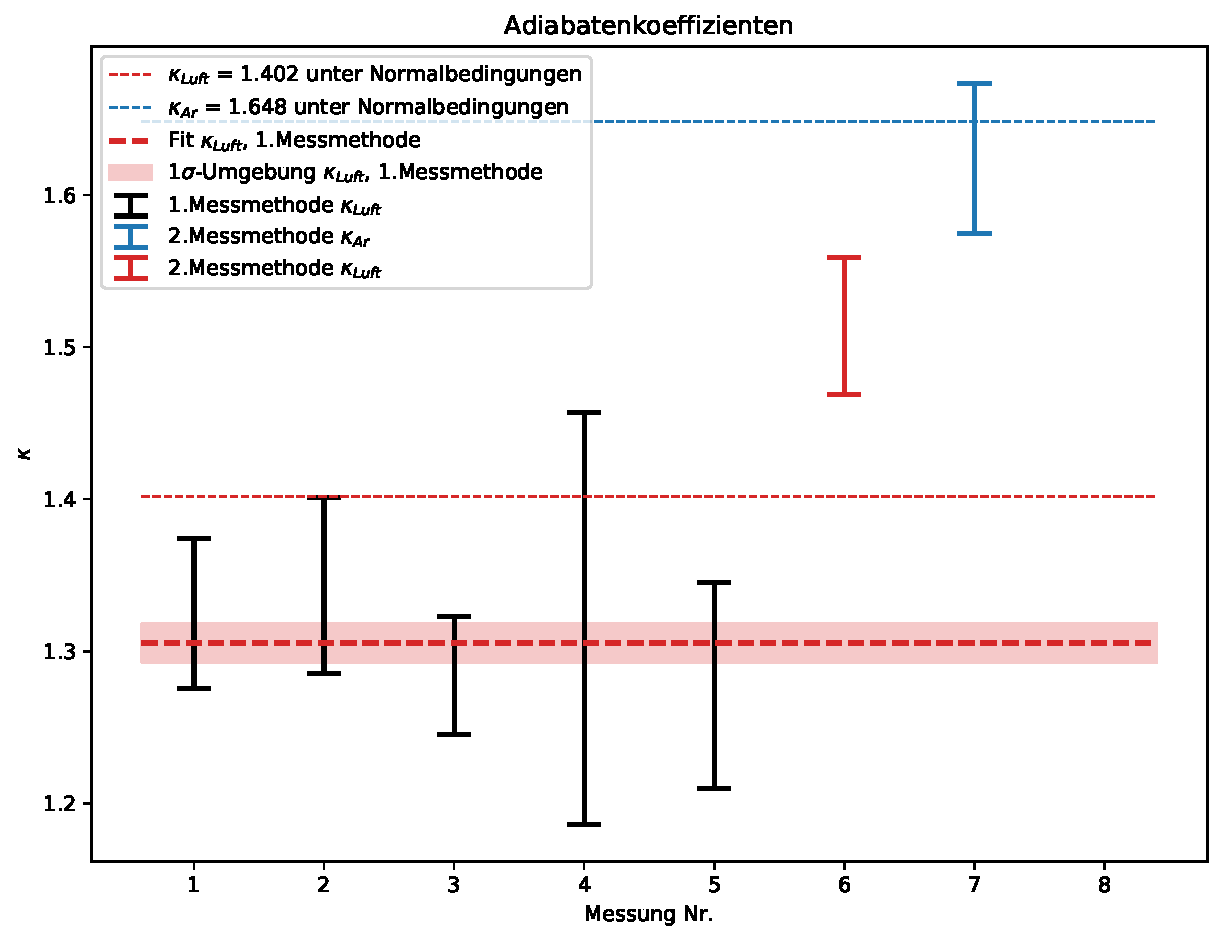
\includegraphics[width=0.8\textwidth]{221_Fig1.pdf}}{1}
  \end{annotate}
\caption{}
\label{fig:Fig1}
\end{figure}
\subsection{Auswertung}
Verglichen mit den Literatur werten \(\kappa_{Luft,Literatur}=1.402(1)\), \(\kappa_{Argon,Literatur}=1.648(1)\) liegt unser Messwert für Argon innerhalb der 1-Sigma Umgebung, der Wert für Luft weicht aber um  \[\frac{{kappa_{Luft,1}}-{kappa_{Luft,Literatur}}}{\Delta {kappa_{Luft,1}}}=2 .2\] ab. Diese 2-Sigma Abweichung kann immer noch von rein  statistischer Natur sein, aber wieder ist nicht ausgeschlossen, dass systematische Fehler, wie das falsche Kalibrieren des Nadelventil an der Apparatur, also eine nicht genug symmetrische Schwingung um die Gasaustrittsöffnung, zum Fehler von 
\[1- \frac{{\kappa_{Luft,1}}}{\kappa_{Luft,Literatur}}\approx +8.0\%\] 
signifikant beitragen konnten.

\section{Fazit}
Unsere Messeergebisse und die Literaturwerte
\begin{align*}
\kappa_{Luft,1}&=1.305(13)\\
\kappa_{Luft,2}&=1.514(45)\\
\kappa_{Argon}&=1.624(49)\\\\
\kappa_{Luft,Literatur}&=1.402(1)\\
\kappa_{Argon,Literatur}&=1.648(1)
\end{align*}
stimmen zwar für Argon überein (weichen nicht signifikant von einander ab, \(< 1\sigma\)) und sind auch für Luft bei der Messung nach Rüchhardt noch im akzeptablen Bereich der statistischen Fehler( \(\approx2.2\sigma\))). Um das weiter zu analysieren müsste der Versuch ausführlicher wiederholt werden.
Bei der Messung des Adiabatenkoeffizienten nach Clément \& Desormes für Luft ist ohne Zweifel ein systematischer Fehler nicht beachtet worden (\(\approx 7.5\sigma\)). Mögliche Gründe hierfür wurden schon  in der Auswertung aufgezählt. Da \(\Delta n = 1\) abgeschätzt wurde, aber es durchaus möglich gewesen ist, das man sich um sogar 2 oder mehr Oszillationen verzählt hat. Bei \(\Delta n = 50\) könnte also ein \(\Delta n \geqslant 2\) den Fehler zum Literaturwert von \(-7.3\%\) auf unter 2-Sigma Signifikanz drücken. Bei einmaliger Durchführung eines solchen Versuchs ist diese Hypothese nicht auszuschließen. Durch weiteres Wiederholen oder mit besserer Abzählmethode könnte dieser Fehler besser bewertet und reduziert werden und gegebenenfalls somit auf andere Quellen für den systematischen Fehler geschlossen werden wie z.B. Luftfeuchtigkeit.
\unboldmath
\end{document}
